% Options for packages loaded elsewhere
\PassOptionsToPackage{unicode}{hyperref}
\PassOptionsToPackage{hyphens}{url}
%
\documentclass[
  preprint]{elsarticle}
\usepackage{amsmath,amssymb}
\usepackage{iftex}
\ifPDFTeX
  \usepackage[T1]{fontenc}
  \usepackage[utf8]{inputenc}
  \usepackage{textcomp} % provide euro and other symbols
\else % if luatex or xetex
  \usepackage{unicode-math} % this also loads fontspec
  \defaultfontfeatures{Scale=MatchLowercase}
  \defaultfontfeatures[\rmfamily]{Ligatures=TeX,Scale=1}
\fi
\usepackage{lmodern}
\ifPDFTeX\else
  % xetex/luatex font selection
\fi
% Use upquote if available, for straight quotes in verbatim environments
\IfFileExists{upquote.sty}{\usepackage{upquote}}{}
\IfFileExists{microtype.sty}{% use microtype if available
  \usepackage[]{microtype}
  \UseMicrotypeSet[protrusion]{basicmath} % disable protrusion for tt fonts
}{}
\makeatletter
\@ifundefined{KOMAClassName}{% if non-KOMA class
  \IfFileExists{parskip.sty}{%
    \usepackage{parskip}
  }{% else
    \setlength{\parindent}{0pt}
    \setlength{\parskip}{6pt plus 2pt minus 1pt}}
}{% if KOMA class
  \KOMAoptions{parskip=half}}
\makeatother
\usepackage{xcolor}
\usepackage{longtable,booktabs,array}
\usepackage{calc} % for calculating minipage widths
% Correct order of tables after \paragraph or \subparagraph
\usepackage{etoolbox}
\makeatletter
\patchcmd\longtable{\par}{\if@noskipsec\mbox{}\fi\par}{}{}
\makeatother
% Allow footnotes in longtable head/foot
\IfFileExists{footnotehyper.sty}{\usepackage{footnotehyper}}{\usepackage{footnote}}
\makesavenoteenv{longtable}
\usepackage{graphicx}
\makeatletter
\def\maxwidth{\ifdim\Gin@nat@width>\linewidth\linewidth\else\Gin@nat@width\fi}
\def\maxheight{\ifdim\Gin@nat@height>\textheight\textheight\else\Gin@nat@height\fi}
\makeatother
% Scale images if necessary, so that they will not overflow the page
% margins by default, and it is still possible to overwrite the defaults
% using explicit options in \includegraphics[width, height, ...]{}
\setkeys{Gin}{width=\maxwidth,height=\maxheight,keepaspectratio}
% Set default figure placement to htbp
\makeatletter
\def\fps@figure{htbp}
\makeatother
\setlength{\emergencystretch}{3em} % prevent overfull lines
\providecommand{\tightlist}{%
  \setlength{\itemsep}{0pt}\setlength{\parskip}{0pt}}
\setcounter{secnumdepth}{5}
\newlength{\cslhangindent}
\setlength{\cslhangindent}{1.5em}
\newlength{\csllabelwidth}
\setlength{\csllabelwidth}{3em}
\newlength{\cslentryspacingunit} % times entry-spacing
\setlength{\cslentryspacingunit}{\parskip}
\newenvironment{CSLReferences}[2] % #1 hanging-ident, #2 entry spacing
 {% don't indent paragraphs
  \setlength{\parindent}{0pt}
  % turn on hanging indent if param 1 is 1
  \ifodd #1
  \let\oldpar\par
  \def\par{\hangindent=\cslhangindent\oldpar}
  \fi
  % set entry spacing
  \setlength{\parskip}{#2\cslentryspacingunit}
 }%
 {}
\usepackage{calc}
\newcommand{\CSLBlock}[1]{#1\hfill\break}
\newcommand{\CSLLeftMargin}[1]{\parbox[t]{\csllabelwidth}{#1}}
\newcommand{\CSLRightInline}[1]{\parbox[t]{\linewidth - \csllabelwidth}{#1}\break}
\newcommand{\CSLIndent}[1]{\hspace{\cslhangindent}#1}
\usepackage{tipa}
\ifLuaTeX
  \usepackage{selnolig}  % disable illegal ligatures
\fi
\IfFileExists{bookmark.sty}{\usepackage{bookmark}}{\usepackage{hyperref}}
\IfFileExists{xurl.sty}{\usepackage{xurl}}{} % add URL line breaks if available
\urlstyle{same}
\hypersetup{
  hidelinks,
  pdfcreator={LaTeX via pandoc}}

\author{}
\date{\vspace{-2.5em}}

\begin{document}

\hypertarget{introduction}{%
\section{Introduction}\label{introduction}}

Perceptual adaptation is a core aspect of language comprehension.
This ability to calibrate the perceptual system in response to novel input allows listeners to map unfamiliar, variable, or secondary acoustic cues onto stable phonetic categories.
Previous research has shown that perceptual adaptation to particular cue-category mappings can transfer from one talker to another (e.g., Kraljic and Samuel 2006, 2007; Reinisch and Holt 2014).
More broadly, the benefits of exposure to an L2 accent can transfer to a new talker with the same accent.
However, there is disagreement in the literature about the conditions under which adaptation generalizes across talkers.
Two different factors have been argued to facilitate generalization: (1) \emph{variability} during exposure (Baese-Berk, Bradlow, and Wright 2013; Bradlow and Bent 2008) and (2) \emph{similarity} between the exposure and test talkers (Xie and Myers 2017; Xie, Liu, and Jaeger 2021).
The present study features three experiments that directly compare variability and similarity during exposure to Spanish-accented English.
The goal is to understand how listeners use acoustic-phonetic information to accommodate linguistic variation.

\hypertarget{l2-accented-speech}{%
\subsection{L2-accented speech}\label{l2-accented-speech}}

During L2 acquisition, a speaker's L1 phonetic inventory shapes the production of L2 speech sounds (Flege and Bohn 2021; for a recent review, see Nagle and Baese-Berk 2022).
This cross-language influence in bilingual speech production is a product of the relations between L1 and L2 phonetic categories (Flege 2007; Flege, Schirru, and MacKay 2003).
These relations determine how an L2 phone is categorized within the L1 phonological system (Best, McRoberts, and Goodell 2001; Best and Tyler 2007).
Here, we focus on a case of two-category assimilation (Best 1994; Tyler et al. 2014), where two contrasting L2 phonemes map onto two contrasting L1 phonemes.
Specifically, we focus on three contrasting phoneme pairs found in both English and Spanish: /p/-/b/ (\emph{park} vs.~\emph{bark}), /t/-/d/ (\emph{tune} vs.~\emph{dune}), and /k/-/g/ (\emph{coal} vs.~\emph{goal}).

These consonant pairs all have the same manner of articulation (stop) but different places of articulation (bilabial, alveolar, and velar, respectively).
Critically, within each pair, one member differs from the other in terms of voicing (voiceless-voiced, respectively).
Voicing refers to the status of the glottis, which comprises two folds of tissue in the larynx at the top of the neck.
Constricting the vocal folds causes them to vibrate, resulting in voiced speech sounds.
By contrast, opening the vocal folds prevents vibration, resulting in voiceless speech sounds.
The consonants /p/, /t/, and /k/ are voiceless, while the consonants /b/, /d/, and /g/ are voiced.
This small articulatory distinction plays an outsized role in the phonological systems of many languages, including English and Spanish.
However, it can be difficult for a listener to detect this contrast in continuous speech.
How, then, can a listener tell the difference between a talker's /p/ and /b/?

Throughout language acquisition, listeners (and speakers themselves) learn which acoustic-phonetic features are most strongly associated with this fine-grained phonological voicing contrast.
There are several interrelated cues that listeners use to distinguish voiced from voiceless stops in word-initial position, including onset fundamental frequency (Whalen et al. 1993), formant transitions (Cooper 1974; Benkí 2001), and vowel duration (Port and Dalby 1982; Viswanathan, Olmstead, and Aivar 2020).
However, the primary cue to word-initial stop consonant voicing is voice onset time (VOT), which is the interval between the release of the closure of the articulators, called the burst, and the beginning of voicing (Lisker and Abramson 1964; Cho and Ladefoged 1999; Chodroff, Golden, and Wilson 2019).
Listeners are highly sensitive to the probabilistic distributions of VOT across voiced and voiceless English stops (Clayards et al. 2008).

The associations between VOT and stop consonants vary cross-linguistically (Chodroff, Golden, and Wilson 2019; Lisker and Abramson 1970).
There are three general types of VOT: lead, where voicing begins before the release, resulting in negative values; short lag, where voicing begins immediately or relatively quickly after the release; and long lag, where voicing begins relatively slowly after the release (Abramson and Whalen 2017).
In Spanish, lead VOTs correspond to voiced stops and short lag VOTs correspond to voiceless stops (Vicente 1986; Williams 1977).
For example, the /b/ in Spanish \emph{barco} (boat) would be approximately -98 ms on average, while the /p/ in Spanish \emph{parque} (park) would be approximately 16 ms on average (values calculated from Chodroff, Golden, and Wilson 2019).
By contrast, in English, short lag VOTs correspond to voiced stops and long lag VOTs correspond to voiceless stops (Chodroff and Wilson 2017).
For example, the /b/ in English \emph{bark} would be approximately 9 ms on average, while the /p/ in English \emph{park} would be approximately 60 ms on average (values calculated from Chodroff, Golden, and Wilson 2019).
In other words, the VOT for Spanish /p/ is a better fit for the contrasting English /b/ phoneme category than for the corresponding English /p/ phoneme category.
The overlap in VOT between Spanish /p/ and English /b/ is illustrated in Figure \ref{fig:intro-fig}, with probability densities constructed from the data presented in Chodroff, Golden, and Wilson (2019).

\begin{figure}

{\centering 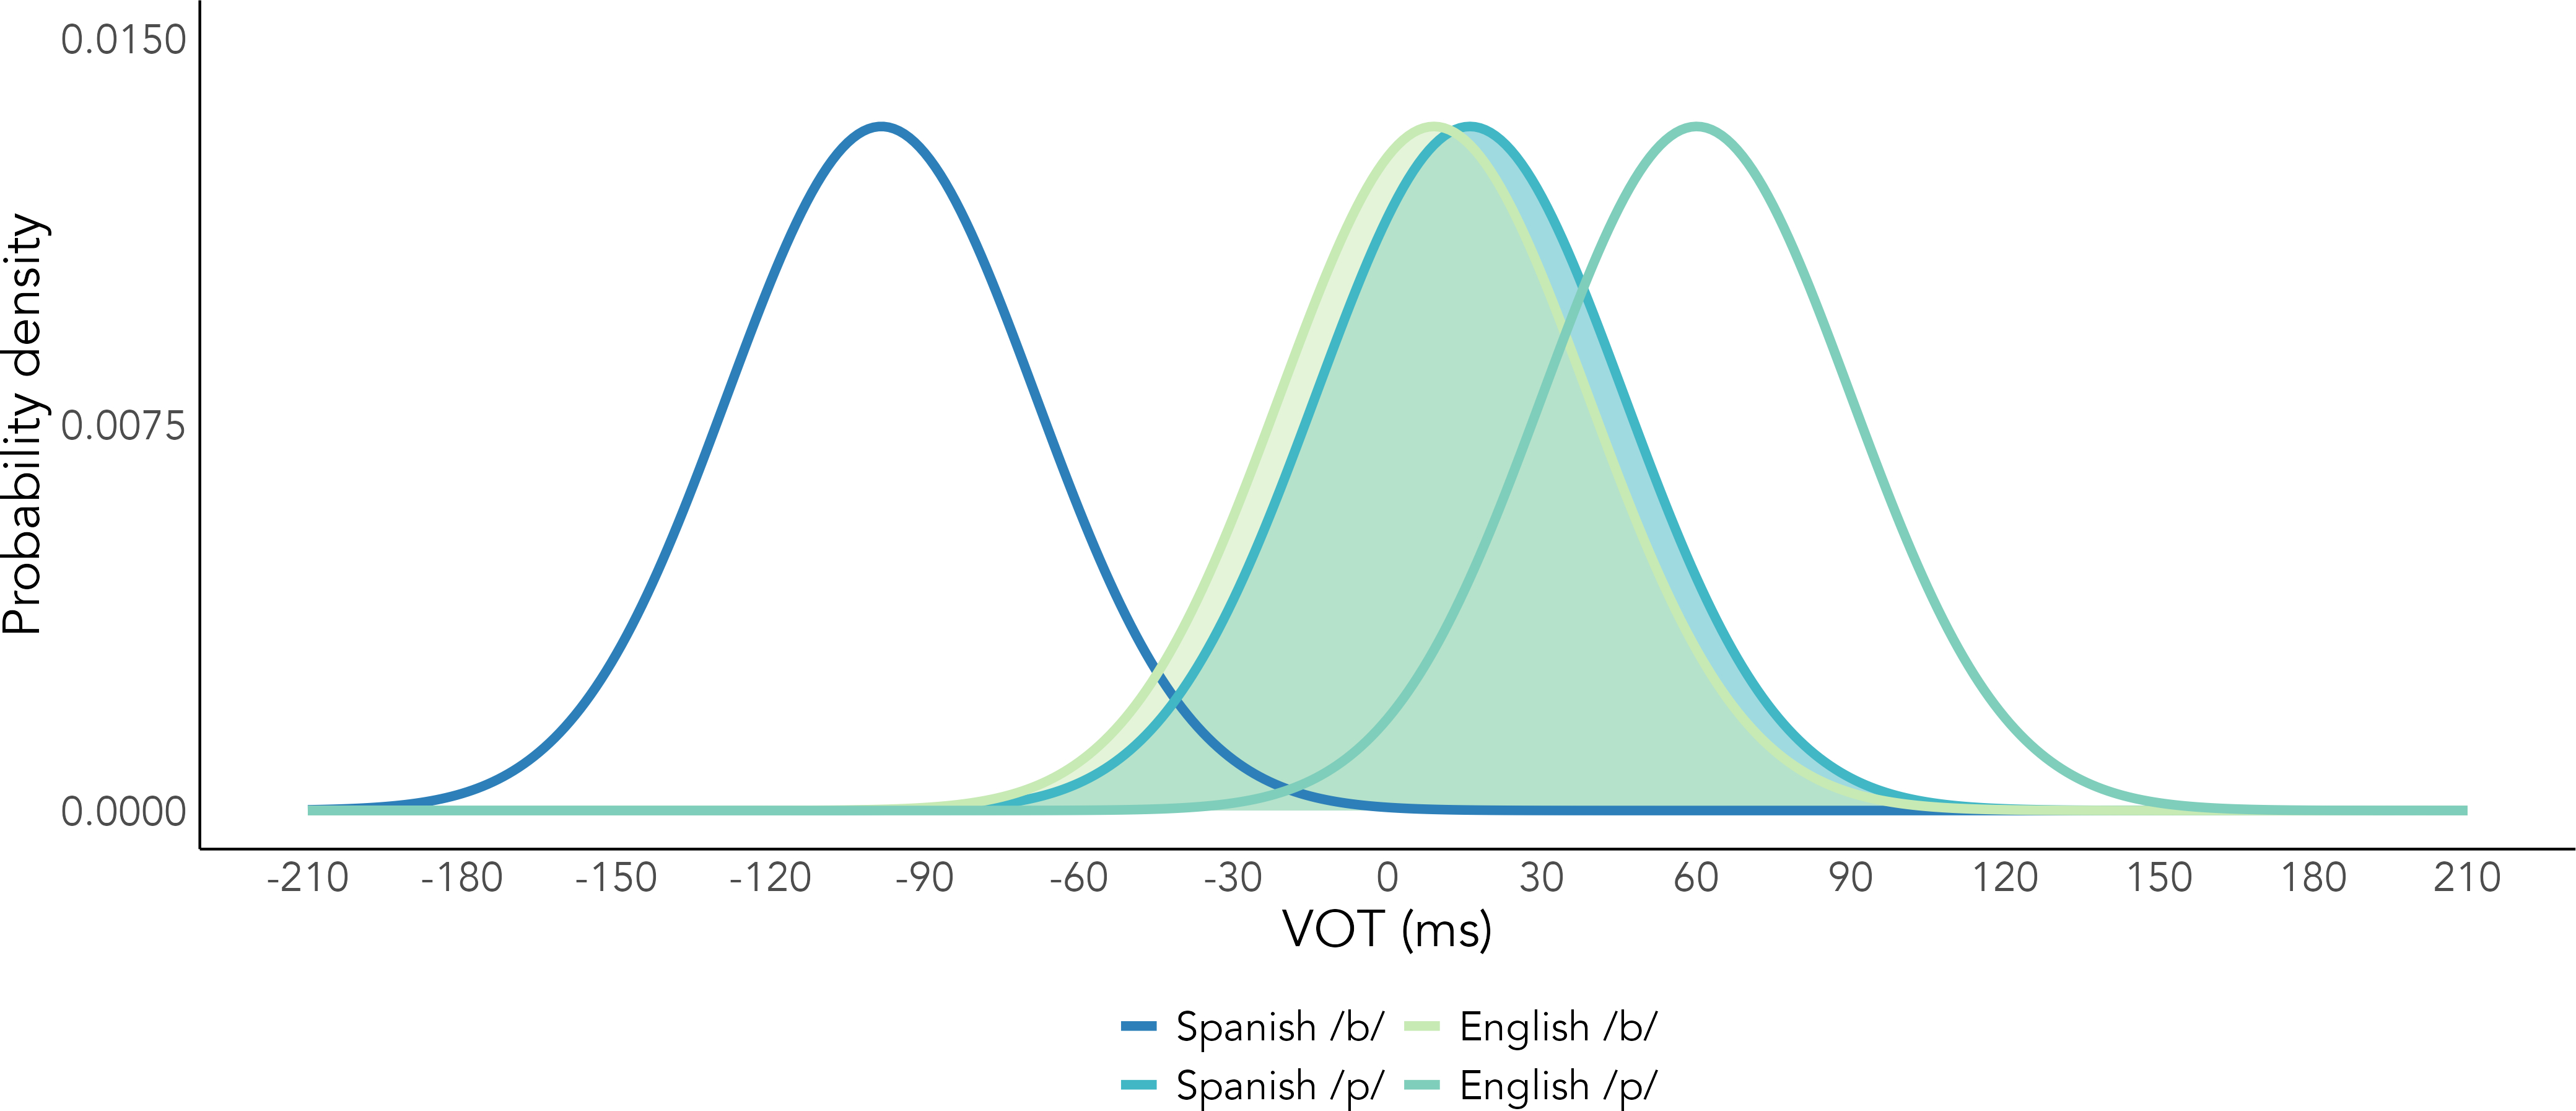
\includegraphics[width=\textwidth]{../14_final_diss/sections/code/outputs/l1_plot} 

}

\caption{Overlapping VOT distributions for Spanish voiceless stops and English voiced stops.}\label{fig:intro-fig}
\end{figure}

To return to the notion of two-category assimilation, consider an L1 Spanish speaker who is learning English as an L2.
She already has an established /p/-/b/ contrast in her L1 Spanish that is associated with VOT.
The /p/-/b/ contrast in her L2 English is associated with the same cue in the same direction, such that VOTs for /p/ are longer than those for /b/.
As a result, the English /p/-/b/ contrast will be relatively easy to integrate into her existing phonological system compared to, for example, certain vowel contrasts in English (Baigorri, Campanelli, and Levy 2019).
The same will be true for both the /t/-/d/ and /k/-/g/ contrasts.
However, assimilating the L2 English /p/ to the L1 Spanish /p/ means that the English phoneme will be produced like the Spanish phoneme.
That is, English /p/ will be produced with a short lag VOT (similar to Spanish /p/).
This will create a perceptual problem from a listener's perspective, since short lag VOTs are associated with English /b/, not /p/; without supporting contextual information, listeners may confuse Spanish-accented English /p/ with /b/ (e.g., \emph{park} perceived as \emph{bark}).
To summarize, cross-language transfer in Spanish-accented English can create ambiguity between voiced and voiceless stops (Flege and Eefting 1987).
Thankfully, listeners are adept at solving this perceptual problem through adaptation.

\hypertarget{adaptation-to-l2-accented-speech}{%
\subsection{Adaptation to L2-accented speech}\label{adaptation-to-l2-accented-speech}}

Perceptual adaptation research shows that listeners quickly orient to the linguistic features of L2-accented speech (Bent and Baese-Berk 2021).
A typical experimental design features an exposure phase, in which participants gain experience with a speech pattern, followed by a test phase.
Talker-specific adaptation is the result of hearing the same talker during exposure and test.
For example, participants who train on Talker A during exposure tend to perform better on Talker A during test than participants who train on Talker B (Bradlow and Bent 2008; Clarke and Garrett 2004; Xie, Liu, and Jaeger 2021; Xie, Theodore, and Myers 2017; Xie et al. 2018; cf. Bradlow, Bassard, and Paller 2023).
Talker-independent adaptation, or generalization, is the result of exposure to a type of talker.
For example, participants who train on Accent X during exposure tend to perform better on Accent X during test than participants who train on Accent Y (Alexander and Nygaard 2019; Bradlow and Bent 2008; Sidaras, Alexander, and Nygaard 2009; Tzeng et al. 2016; Xie, Liu, and Jaeger 2021; Xie et al. 2018).
Overall, experience with L2-accented talkers improves perception of novel L2-accented talkers (Witteman, Weber, and McQueen 2013; Tzeng, Russell, and Nygaard 2024; Reinisch and Holt 2014; Bieber and Gordon-Salant 2022; Baese-Berk, Bradlow, and Wright 2013).

\hypertarget{talker-independent-adaptation-to-l2-accented-speech}{%
\subsubsection{Talker-independent adaptation to L2-accented speech}\label{talker-independent-adaptation-to-l2-accented-speech}}

The pattern of results for talker-independent adaptation becomes more complicated when considering different types of exposure to an accent.
Studies often compare single-talker exposure, in which one talker produces all of the stimuli for a condition, to multi-talker exposure, in which several different talkers produce the stimuli for a condition.
For example, participants in a single-talker exposure condition listen to Talker A with Accent X and participants in a multi-talker exposure condition listen to Talkers B, C, and D with Accent X.
During test, both groups listen to Talker E with Accent X.
Differences in task performance with Talker E index generalization from exposure (Baese-Berk, Bradlow, and Wright 2013; Bradlow and Bent 2008; Xie and Myers 2017; Xie, Liu, and Jaeger 2021).

Experiment 2 of Bradlow and Bent (2008) illustrates how exposure generalizes across L2-accented talkers with the same L1.
In this experiment, participants completed a sentence transcription task during both exposure and test, and performance was measured in terms of sentence recognition accuracy.
There were four key exposure conditions: multi-talker, single-talker, and control.
Participants in the multi-talker condition were exposed to five different Mandarin-accented English talkers, while those in the single-talker condition were exposed to just one Mandarin-accented English talker.
Control training featured five L1-accented English talkers.
Training was followed by two post-tests: one featured a novel talker with a familiar L2 accent (Mandarin) and the other featured a novel talker with an unfamiliar L2 accent (Slovakian).
Performance on the Mandarin-accented English test talker was higher in the multi-talker condition than in the single-talker or control conditions.
By contrast, performance on the Slovakian-accented English test talker did not differ between conditions.
These results suggest that exposure to multiple talkers highlights the characteristic features of an L2 accent, which in turn helps listeners adapt to novel talkers with the same accent.

Baese-Berk, Bradlow, and Wright (2013) provided evidence that exposure to multiple L2-accented talkers with \emph{different} L1s also facilitates generalization.
They used the same stimulus materials and procedures as Experiment 2 in Bradlow and Bent (2008) in order to compare a multi-accent exposure group directly to the multi-talker exposure and control groups from the previous study.
During multi-accent training, participants were exposed to five L2-accented English talkers, each of whom had a different L1: Thai, Korean, Hindi, Romanian, and Mandarin.
Multi-accent and multi-talker exposure were equally effective at facilitating talker-independent adaptation to the Mandarin-accented test talker relative to control exposure.
Critically, multi-accent exposure also generalized to the Slovakian-accented test talker, while multi-talker and control exposure did not.
Together, these results suggest that exposure to multiple accents highlights the overall features shared by L2 speakers of English.
This experience in turn helps listeners adapt to novel talkers not only with familiar accents, but also with unfamiliar accents.

Xie, Liu, and Jaeger (2021) investigated the conditions under which single-talker exposure can facilitate generalization.
Specifically, they sought to replicate Bradlow and Bent (2008) with one key change: counterbalancing the test and exposure talkers.
In the original study, different (partially overlapping) sets of Mandarin-accented English talkers were used in the multi-talker and single-talker exposure conditions.
Thus, the lack of generalization from single-talker training may have been the result of the specific talkers, rather than the superiority of multi-talker exposure per se.
The specific combination of exposure and test talkers is likely to have affected performance under both exemplar-based (e.g., Goldinger 1998; Johnson 2006), and hybrid (e.g., Pierrehumbert 2016; Kleinschmidt and Jaeger 2015) models of speech perception (see Introduction to Xie, Liu, and Jaeger 2021).
To address this potential confound, Xie, Liu, and Jaeger (2021) used a single set of Mandarin-accented talkers for both multi-talker and single-talker exposure; in addition, these talkers were rotated through the exposure talker and test talker roles.
The results replicated Bradlow and Bent (2008)'s finding that multi-talker exposure facilitates generalization more than control exposure.
However, contrary to Bradlow and Bent (2008), they found that single-talker exposure also facilitated generalization more than control exposure.
When comparing multi- and single-talker exposure, the difference in performance depended on the particular combination of exposure and test talkers.
Overall, these results suggest that generalization is strongly influenced by talker-specific features.

Xie and Myers (2017) investigated the acoustic-phonetic features of the exposure talkers that facilitate generalization.
In this study, participants were exposed to Mandarin-accented English through an auditory lexical decision task.
Experimental exposure included multisyllabic real words that biased listeners toward perceiving ambiguous word-final stops as /d/ rather than as /t/ (e.g., \emph{overload}).
Control exposure did not include these critical items.
Both types of exposure featured five Mandarin-accented talkers; the only difference was in the presence of disambiguating lexical contexts for learning ambiguous word-final /d/.
During test, participants performed a primed cross-modal lexical decision task with a novel Mandarin-accented talker.
Previous exposure to Mandarin-accented word-final English /d/ in disambiguating lexical contexts generalized to the novel talker.
Specifically, lexical activation for the /d/-final member of minimal pairs like \emph{seed} versus \emph{seat} was increased in the experimental versus the control group.
The results suggest that listeners did not simply expand their phonetic category boundaries with exposure; instead, they used the lexical contexts from training to re-tune their categories for particular accented features.

Two follow-up experiments with single-talker exposure revealed the importance of exposure-test similarity.
Of the five talkers included in the multi-talker exposure, two were selected.
The first talker was the dissimilar talker, who differed from the test talker on the three key acoustic measures associated with the word-final /t/-/d/ contrast.
The second talker was the similar talker, who did not differ from the test talker in the means of these measures.
Exposure to the similar talker generalized to the test talker, with experimental exposure decreasing lexical competition between \emph{seed}-\emph{seat} minimal pairs compared to control exposure.
By contrast, exposure to the dissimilar talker did not increase performance relative to control exposure.
Moreover, generalization from the similar talker was as strong as generalization from multi-talker exposure (which included the similar talker).
Together, the results of Xie and Myers (2017) show that the correspondence between exposure and test talkers at the acoustic-phonetic level is critical for understanding the observed patterns of generalization across studies.

\hypertarget{competing-hypotheses-for-generalization}{%
\subsubsection{Competing hypotheses for generalization}\label{competing-hypotheses-for-generalization}}

There are two competing explanations for why multi-talker exposure may or may not provide additional benefits for generalization over single-talker exposure: the exposure-to-variability hypothesis and the similarity-based hypothesis.

On the one hand, the exposure-to-variability hypothesis posits that L2-accented talkers exhibit similarities in production that differ from L1-accented norms (Baese-Berk, Bradlow, and Wright 2013).
The exposure-to-variability hypothesis also posits that among L2-accented talkers with the \emph{same L1}, cross-language influence shifts the relations between acoustic cues and phonetic categories similarly across talkers.
Among L2-accented talkers with \emph{different L1s}, typological features that are unique to the L2 lead to similarly accented realizations regardless of the L1.
Multi-talker exposure thus allows listeners to abstract away from the peculiarities of any given talker and home in on these commonalities.
For example, a listener encountering one unfamiliar Spanish-accented talker may not know whether their short lag VOTs are specific to that talker or characteristic of the L2 accent.
By contrast, a listener encountering multiple unfamiliar Spanish-accented talkers at once would not only see that short lag VOTs are common across the talkers, but also that other accent features (e.g., vowel height) exhibit covariation with voicing (Clayards 2017).
In Bradlow and Bent (2008), multi-talker exposure outperformed single-talker exposure, suggesting that training on multiple L2-accented talkers (with the same L1) allowed listeners to separate the characteristic features of an accent from the idiosyncratic features of a talker.
The results of Bradlow and Bent (2008) support the exposure-to-variability hypothesis, but do not align with the effects observed by Xie and Myers (2017) and Xie, Liu, and Jaeger (2021).

On the other hand, the similarity-based hypothesis posits that acoustic-phonetic overlap between the exposure and test talkers, rather than variability during exposure, facilitates generalization (Xie, Liu, and Jaeger 2021).
In Xie and Myers (2017), listeners exhibited comparable talker-independent adaptation effects after both single- and multi-talker exposure to Mandarin-accented realizations of word-final /d/, which is perceptually confusable with /t/ (e.g., \emph{seed} vs.~\emph{seat}).
Critically, both exposure conditions contained a Mandarin-accented talker with similar word-final /d/ acoustics to the test talker.
Xie, Liu, and Jaeger (2021) also demonstrated equivalent generalization effects from single- and multi-talker exposure to Mandarin-accented speech.
They argue that exposure to multiple talkers merely increases the likelihood that listeners will encounter a cue distribution that is relevant for adapting to the test talker.
For example, multi-talker training on Spanish-accented speech is more likely to include at least one talker with short lag VOTs than single-talker training.
Bradlow and Bent (2008)'s multi-talker exposure condition may have included talkers who were more similar to the test talker than their single-talker exposure condition, which would confound talker similarity and exposure to variability.
Xie, Liu, and Jaeger (2021) addressed this confound by counterbalancing the combinations of exposure and test talkers across participants.
Thus, the similarity-based hypothesis may account for the differential effects of single- and multi-talker exposure in perceptual adaptation studies, but further research is needed to distinguish the roles of variability and similarity in talker-independent adaptation.
To summarize, the similarity-based hypothesis focuses on specific cue-category mappings, while the exposure-to-variability hypothesis focuses on the covariation between cues.

\hypertarget{comparing-variability-and-similarity}{%
\subsection{Comparing variability and similarity}\label{comparing-variability-and-similarity}}

As discussed above, the results of Bradlow and Bent (2008) support the exposure-to-variability hypothesis, while those of Xie and Myers (2017) and Xie, Liu, and Jaeger (2021) support the similarity-based hypothesis.
We argue that the socio-indexical structure of cue-category mappings in the ideal adapter framework provides a link between these two hypotheses and can account for these conflicting findings (Kleinschmidt 2019).
According to this theory, listeners represent each cue-category mapping according to informative and useful groupings.
For L2-accented speech, these groupings may be structured according to each talker (talker-specific) or to the L2 accent shared by the talkers (talker-independent).

The exposure-to-variability hypothesis argues that increasing variability during exposure increases systematic covariation among relevant cues, enabling listeners to separate the idiosyncratic features of a talker from the common features of an accent.
To restate this hypothesis in terms of the ideal adapter framework, covariation among individual exposure talkers promotes the development of a robust talker-independent model (or refinement of an existing one).
In turn, this talker-independent model guides adaptation to the novel test talker.
This exposure-to-variability perspective assumes that talker-independent models are better for generalization than talker-specific models.

By contrast, the similarity-based hypothesis argues that increasing the similarity between the cue-category mappings of the exposure and test talkers facilitates generalization.
Translating this hypothesis into the ideal adapter framework, listeners develop robust talker-specific models during exposure.
During test, listeners use the model that provides the most information about the test talker's cue distributions and most readily predicts their individual cue values to guide adaptation.
This similarity-based perspective assumes that talker-specific models are best for generalization because they provide precise information about cue-category mappings.

Overall, the specificity of a listener's set of generative models may explain the effects of variability and similarity on generalization.
The present study tests these two hypotheses in order to probe the mechanisms underlying adaptation to L2-accented speech.
The overarching goal is to understand how the L1 speech recognition system learns the patterns of cross-language influence in L2 speech production.

\hypertarget{present-study}{%
\subsection{Present study}\label{present-study}}

How do listeners generalize their experience with L2-accented speech?
On the one hand, the \emph{structure} of exposure may be the primary driver of talker-independent adaptation.
Variability has been the primary focus of structural inquiries (Baese-Berk, Bradlow, and Wright 2013), with the number of talkers being the key manipulation (Bradlow and Bent 2008; Bieber and Gordon-Salant 2022; Choi and Perrachione 2019; Xie, Liu, and Jaeger 2021).
On the other hand, the \emph{content} of exposure may be the key to effective generalization.
At a high level, training on the relevant L2 accent tends to facilitate talker-independent adaptation (Bradlow, Bassard, and Paller 2023; Clarke and Garrett 2004; Xie et al. 2018; Alexander and Nygaard 2019).
At a detailed level, exposure to the relevant acoustic-phonetic features of an L2 accent explains generalization beyond shared L1 (Xie and Myers 2017; Sidaras, Alexander, and Nygaard 2009; Reinisch and Holt 2014).
Together, a shared L1 and common acoustic-phonetic features create similarity between exposure and test talkers that facilitates adaptation.
The present study builds on this body of work investigating generalization of L2-accented speech.
The key difference between our study and earlier work is the operationalization of variability and similarity.
Specifically, we increased the precision with which variability was implemented (c.f. Baese-Berk, Bradlow, and Wright 2013) and expanded the scope of similarity (c.f. Xie and Myers 2017) in order to better delineate the exposure-to-variability and similarity-based hypotheses.
The goal was to clarify some of the inconsistent findings in the literature for talker-independent adaptation to L2-accented speech (Bent and Baese-Berk 2021).

Regarding variability, previous studies have almost exclusively investigated this factor as a comparison between single-talker exposure and multi-talker exposure (c.f. Baese-Berk, Bradlow, and Wright 2013; Bradlow, Bassard, and Paller 2023).
However, multi-talker exposure reduces the amount of experience with any given talker relative to single-talker exposure.
From the larger perceptual adaptation literature, we know that listeners are highly sensitive to acoustic-phonetic mappings and use them to adapt to new talkers (e.g., Kraljic and Samuel 2006).
We also know that there is a high degree of within- and between-talker variability in both L1- and L2-accented speech production (Xie and Jaeger 2020; Wade, Jongman, and Sereno 2007).
Depending on the idiosyncrasies of a given exposure talker, altering the amount of experience with this talker may benefit or impede generalization.
This asymmetry in talker-specific exposure may explain some of the inconsistent findings in the literature (Xie and Myers 2017; Xie, Liu, and Jaeger 2021).
Moreover, exposure to multiple talkers increases the sources of covariation to account for, which in turn increases the difficulty of accounting for them during exposure.
If we assume, as the exposure-to-variability hypothesis does, that experience with covariation is critical for generalization, this lack of clarity obscures how and why variability might facilitate generalization.
In the present study, we used a single group of talkers with the same L1 to control the type and amount of experience with each talker across levels of variability.

Regarding similarity, previous studies have either conceptualized this factor at the accent level or at the acoustic-phonetic level.
When it comes to operationalizing either definition of similarity, we run into the same problem as we did with multi-talker versus single-talker exposure.
That is, we end up comparing two (or more) groups of exposure talkers between conditions.
If we assume again that listeners are highly sensitive to talker-specific acoustic-phonetic features, then this design confounds talker- and accent-specific effects.
In other words, we cannot know whether listeners are ``learning a talker or learning an accent'' or learning both (Xie and Myers 2017).
Here, we manipulated the stimuli listeners encounter during exposure rather than the talkers in order to maintain consistency across levels of similarity.
Moreover, we directly crossed the factors of similarity and variability in the same design, which, to our knowledge, has not yet been done.
Overall, this study allows us to address the ongoing debate between the exposure-to-variability and similarity-based hypotheses for generalization.

\newpage

\section*{References}

\setlength{\parindent}{-0.2in}
\setlength{\leftskip}{0.2in}

\noindent

\hypertarget{refs}{}
\begin{CSLReferences}{1}{0}
\leavevmode\vadjust pre{\hypertarget{ref-abramson2017}{}}%
Abramson, Arthur S, and Douglas H Whalen. 2017. {``Voice Onset Time ({VOT}) at 50: Theoretical and Practical Issues in Measuring Voicing Distinctions.''} \emph{Journal of Phonetics} 63: 75--86.

\leavevmode\vadjust pre{\hypertarget{ref-alexander2019}{}}%
Alexander, Jessica E. D., and Lynne C Nygaard. 2019. {``Specificity and Generalization in Perceptual Adaptation to Accented Speech.''} \emph{The Journal of the Acoustical Society of America} 145 (6): 3382--98.

\leavevmode\vadjust pre{\hypertarget{ref-baese2013}{}}%
Baese-Berk, Melissa M, Ann R Bradlow, and Beverly A Wright. 2013. {``Accent-Independent Adaptation to Foreign Accented Speech.''} \emph{The Journal of the Acoustical Society of America} 133 (3): EL174--80.

\leavevmode\vadjust pre{\hypertarget{ref-baigorri2019}{}}%
Baigorri, Miriam, Luca Campanelli, and Erika S Levy. 2019. {``Perception of {American}--{English} Vowels by Early and Late {Spanish}--{English} Bilinguals.''} \emph{Language and Speech} 62 (4): 681--700.

\leavevmode\vadjust pre{\hypertarget{ref-benki2001}{}}%
Benkí, José R. 2001. {``Place of Articulation and First Formant Transition Pattern Both Affect Perception of Voicing in {English}.''} \emph{Journal of Phonetics} 29 (1): 1--22.

\leavevmode\vadjust pre{\hypertarget{ref-bent2021}{}}%
Bent, Tessa, and Melissa Baese-Berk. 2021. {``Perceptual Learning of Accented Speech.''} In, edited by Jennifer S. Pardo, Lynne C. Nygaard, Robert E. Remez, and David B. Pisoni, 428--64. Wiley Blackwell.

\leavevmode\vadjust pre{\hypertarget{ref-best1994}{}}%
Best, Catherine T. 1994. {``The Emergence of Native-Language Phonological Influences in Infants: A Perceptual Assimilation Model.''} \emph{The Development of Speech Perception: The Transition from Speech Sounds to Spoken Words} 167 (224): 233--77.

\leavevmode\vadjust pre{\hypertarget{ref-best2001}{}}%
Best, Catherine T, Gerald W McRoberts, and Elizabeth Goodell. 2001. {``Discrimination of Non-Native Consonant Contrasts Varying in Perceptual Assimilation to the Listener's Native Phonological System.''} \emph{The Journal of the Acoustical Society of America} 109 (2): 775--94.

\leavevmode\vadjust pre{\hypertarget{ref-best2007}{}}%
Best, Catherine T, and Michael Tyler. 2007. {``Second Language Speech Learning: The Role of Language Experience in Speech Perception and Production.''} In, edited by O Bohn and Murray Munro, 13--34. John Benjamins.

\leavevmode\vadjust pre{\hypertarget{ref-bieber2022}{}}%
Bieber, Rebecca E, and Sandra Gordon-Salant. 2022. {``Semantic Context and Stimulus Variability Independently Affect Rapid Adaptation to Non-Native English Speech in Young Adults.''} \emph{The Journal of the Acoustical Society of America} 151 (1): 242--55.

\leavevmode\vadjust pre{\hypertarget{ref-bradlow2023}{}}%
Bradlow, Ann R, Adrianna M Bassard, and Ken A Paller. 2023. {``Generalized Perceptual Adaptation to Second-Language Speech: Variability, Similarity, and Intelligibility.''} \emph{The Journal of the Acoustical Society of America} 154 (3): 1601--13.

\leavevmode\vadjust pre{\hypertarget{ref-bradlow2008}{}}%
Bradlow, Ann R, and Tessa Bent. 2008. {``Perceptual Adaptation to Non-Native Speech.''} \emph{Cognition} 106 (2): 707--29.

\leavevmode\vadjust pre{\hypertarget{ref-cho1999}{}}%
Cho, Taehong, and Peter Ladefoged. 1999. {``Variation and Universals in {VOT}: Evidence from 18 Languages.''} \emph{Journal of Phonetics} 27 (2): 207--29.

\leavevmode\vadjust pre{\hypertarget{ref-chodroff2019}{}}%
Chodroff, Eleanor, Alessandra Golden, and Colin Wilson. 2019. {``Covariation of Stop Voice Onset Time Across Languages: Evidence for a Universal Constraint on Phonetic Realization.''} \emph{The Journal of the Acoustical Society of America} 145 (1): EL109--15.

\leavevmode\vadjust pre{\hypertarget{ref-chodroff2017}{}}%
Chodroff, Eleanor, and Colin Wilson. 2017. {``Structure in Talker-Specific Phonetic Realization: Covariation of Stop Consonant {VOT in American English}.''} \emph{Journal of Phonetics} 61: 30--47.

\leavevmode\vadjust pre{\hypertarget{ref-choi2019}{}}%
Choi, Ja Young, and Tyler K Perrachione. 2019. {``Time and Information in Perceptual Adaptation to Speech.''} \emph{Cognition} 192: 103982.

\leavevmode\vadjust pre{\hypertarget{ref-clarke2004}{}}%
Clarke, Constance M, and Merrill F Garrett. 2004. {``Rapid Adaptation to Foreign-Accented {English}.''} \emph{The Journal of the Acoustical Society of America} 116 (6): 3647--58.

\leavevmode\vadjust pre{\hypertarget{ref-clayards2017}{}}%
Clayards, Meghan. 2017. {``Individual Talker and Token Covariation in the Production of Multiple Cues to Stop Voicing.''} \emph{Phonetica} 75 (1): 1--23.

\leavevmode\vadjust pre{\hypertarget{ref-clayards2008}{}}%
Clayards, Meghan, Michael K Tanenhaus, Richard N Aslin, and Robert A Jacobs. 2008. {``Perception of Speech Reflects Optimal Use of Probabilistic Speech Cues.''} \emph{Cognition} 108 (3): 804--9.

\leavevmode\vadjust pre{\hypertarget{ref-cooper1974}{}}%
Cooper, William E. 1974. {``Selective Adaptation for Acoustic Cues of Voicing in Initial Stops.''} \emph{Journal of Phonetics} 2 (4): 303--13.

\leavevmode\vadjust pre{\hypertarget{ref-flege2007}{}}%
Flege, James E. 2007. {``Language Contact in Bilingualism: Phonetic System Interactions.''} \emph{Laboratory Phonology} 9 (353-381).

\leavevmode\vadjust pre{\hypertarget{ref-flege2021}{}}%
Flege, James E, and O Bohn. 2021. {``The Revised Speech Learning Model (SLM-r).''} \emph{Second Language Speech Learning: Theoretical and Empirical Progress}, 3--83.

\leavevmode\vadjust pre{\hypertarget{ref-flege1987}{}}%
Flege, James E, and Wieke Eefting. 1987. {``Production and Perception of English Stops by Native Spanish Speakers.''} \emph{Journal of Phonetics} 15 (1): 67--83.

\leavevmode\vadjust pre{\hypertarget{ref-flege2003}{}}%
Flege, James E, Carlo Schirru, and Ian R. A. MacKay. 2003. {``Interaction Between the Native and Second Language Phonetic Subsystems.''} \emph{Speech Communication} 40 (4): 467--91.

\leavevmode\vadjust pre{\hypertarget{ref-goldinger1998}{}}%
Goldinger, Stephen D. 1998. {``Echoes of Echoes? An Episodic Theory of Lexical Access.''} \emph{Psychological Review} 105 (2): 251.

\leavevmode\vadjust pre{\hypertarget{ref-johnson2006}{}}%
Johnson, Keith. 2006. {``Resonance in an Exemplar-Based Lexicon: The Emergence of Social Identity and Phonology.''} \emph{Journal of Phonetics} 34 (4): 485--99.

\leavevmode\vadjust pre{\hypertarget{ref-kleinschmidt2019}{}}%
Kleinschmidt, Dave F. 2019. {``Structure in Talker Variability: How Much Is There and How Much Can It Help?''} \emph{Language, Cognition and Neuroscience} 34 (1): 43--68.

\leavevmode\vadjust pre{\hypertarget{ref-kleinschmidt2015}{}}%
Kleinschmidt, Dave F, and T Florian Jaeger. 2015. {``Robust Speech Perception: Recognize the Familiar, Generalize to the Similar, and Adapt to the Novel.''} \emph{Psychological Review} 122 (2): 148.

\leavevmode\vadjust pre{\hypertarget{ref-kraljic2006}{}}%
Kraljic, Tanya, and Arthur G Samuel. 2006. {``Generalization in Perceptual Learning for Speech.''} \emph{Psychonomic Bulletin \& Review} 13 (2): 262--68.

\leavevmode\vadjust pre{\hypertarget{ref-kraljic2007}{}}%
---------. 2007. {``Perceptual Adjustments to Multiple Speakers.''} \emph{Journal of Memory and Language} 56 (1): 1--15.

\leavevmode\vadjust pre{\hypertarget{ref-lisker1964}{}}%
Lisker, Leigh, and Arthur S Abramson. 1964. {``A Cross-Language Study of Voicing in Initial Stops: Acoustical Measurements.''} \emph{Word} 20 (3): 384--422.

\leavevmode\vadjust pre{\hypertarget{ref-lisker1970}{}}%
---------. 1970. {``The Voicing Dimension: Some Experiments in Comparative Phonetics.''} In \emph{Proceedings of the 6th International Congress of Phonetic Sciences}, 563--67.

\leavevmode\vadjust pre{\hypertarget{ref-nagle2022}{}}%
Nagle, Charles L, and Melissa M Baese-Berk. 2022. {``Advancing the State of the Art in L2 Speech Perception-Production Research: Revisiting Theoretical Assumptions and Methodological Practices.''} \emph{Studies in Second Language Acquisition} 44 (2): 580--605.

\leavevmode\vadjust pre{\hypertarget{ref-pierrehumbert2016}{}}%
Pierrehumbert, Janet B. 2016. {``Phonological Representation: Beyond Abstract Versus Episodic.''} \emph{Annual Review of Linguistics} 2: 33--52.

\leavevmode\vadjust pre{\hypertarget{ref-port1982}{}}%
Port, Robert F, and Jonathan Dalby. 1982. {``Consonant/Vowel Ratio as a Cue for Voicing in English.''} \emph{Perception \& Psychophysics} 32: 141--52.

\leavevmode\vadjust pre{\hypertarget{ref-reinisch2014}{}}%
Reinisch, Eva, and Lori L Holt. 2014. {``Lexically Guided Phonetic Retuning of Foreign-Accented Speech and Its Generalization.''} \emph{Journal of Experimental Psychology: Human Perception and Performance} 40 (2): 539.

\leavevmode\vadjust pre{\hypertarget{ref-sidaras2009}{}}%
Sidaras, Sabrina K, Jessica E. D. Alexander, and Lynne C Nygaard. 2009. {``Perceptual Learning of Systematic Variation in {Spanish-accented} Speech.''} \emph{The Journal of the Acoustical Society of America} 125 (5): 3306--16.

\leavevmode\vadjust pre{\hypertarget{ref-tyler2014}{}}%
Tyler, Michael D, Catherine T Best, Alice Faber, and Andrea G Levitt. 2014. {``Perceptual Assimilation and Discrimination of Non-Native Vowel Contrasts.''} \emph{Phonetica} 71 (1): 4--21.

\leavevmode\vadjust pre{\hypertarget{ref-tzeng2016}{}}%
Tzeng, Christina Y, Jessica E. D. Alexander, Sabrina K Sidaras, and Lynne C Nygaard. 2016. {``The Role of Training Structure in Perceptual Learning of Accented Speech.''} \emph{Journal of Experimental Psychology: Human Perception and Performance} 42 (11): 1793.

\leavevmode\vadjust pre{\hypertarget{ref-tzeng2024}{}}%
Tzeng, Christina Y, Marissa L Russell, and Lynne C Nygaard. 2024. {``Attention Modulates Perceptual Learning of Non-Native-Accented Speech.''} \emph{Attention, Perception, \& Psychophysics} 86 (1): 339--53.

\leavevmode\vadjust pre{\hypertarget{ref-vicente1986}{}}%
Vicente, M Luisa Castañeda. 1986. {``El {VOT} de Las Oclusivas Sordas y Sonoras Espa{ñ}olas.''} \emph{Estudios de Fon{é}tica Experimental}, 91--110.

\leavevmode\vadjust pre{\hypertarget{ref-viswanathan2020}{}}%
Viswanathan, Navin, Annie J Olmstead, and M Pilar Aivar. 2020. {``The Use of Vowel Length in Making Voicing Judgments by Native Listeners of {English and Spanish}: Implications for Rate Normalization.''} \emph{Language and Speech} 63 (2): 436--52.

\leavevmode\vadjust pre{\hypertarget{ref-wade2007}{}}%
Wade, Travis, Allard Jongman, and Joan Sereno. 2007. {``Effects of Acoustic Variability in the Perceptual Learning of Non-Native-Accented Speech Sounds.''} \emph{Phonetica} 64 (2-3): 122--44.

\leavevmode\vadjust pre{\hypertarget{ref-whalen1993}{}}%
Whalen, Douglas H, Arthur S Abramson, Leigh Lisker, and Maria Mody. 1993. {``F0 Gives Voicing Information Even with Unambiguous Voice Onset Times.''} \emph{The Journal of the Acoustical Society of America} 93 (4): 2152--59.

\leavevmode\vadjust pre{\hypertarget{ref-williams1977}{}}%
Williams, Lee. 1977. {``The Voicing Contrast in {Spanish}.''} \emph{Journal of Phonetics} 5 (2): 169--84.

\leavevmode\vadjust pre{\hypertarget{ref-witteman2013}{}}%
Witteman, Marijt J, Andrea Weber, and James M McQueen. 2013. {``Foreign Accent Strength and Listener Familiarity with an Accent Codetermine Speed of Perceptual Adaptation.''} \emph{Attention, Perception, \& Psychophysics} 75 (3): 537--56.

\leavevmode\vadjust pre{\hypertarget{ref-xie2020}{}}%
Xie, Xin, and T Florian Jaeger. 2020. {``Comparing Non-Native and Native Speech: Are L2 Productions More Variable?''} \emph{The Journal of the Acoustical Society of America} 147 (5): 3322--47.

\leavevmode\vadjust pre{\hypertarget{ref-xie2021}{}}%
Xie, Xin, Linda Liu, and T Florian Jaeger. 2021. {``Cross-Talker Generalization in the Perception of Nonnative Speech: A Large-Scale Replication.''} \emph{Journal of Experimental Psychology: General}.

\leavevmode\vadjust pre{\hypertarget{ref-xie2017similarity}{}}%
Xie, Xin, and Emily B Myers. 2017. {``Learning a Talker or Learning an Accent: Acoustic Similarity Constrains Generalization of Foreign Accent Adaptation to New Talkers.''} \emph{Journal of Memory and Language} 97: 30--46.

\leavevmode\vadjust pre{\hypertarget{ref-xie2017structure}{}}%
Xie, Xin, Rachel M Theodore, and Emily B Myers. 2017. {``More Than a Boundary Shift: Perceptual Adaptation to Foreign-Accented Speech Reshapes the Internal Structure of Phonetic Categories.''} \emph{Journal of Experimental Psychology: Human Perception and Performance} 43 (1): 206.

\leavevmode\vadjust pre{\hypertarget{ref-xie2018}{}}%
Xie, Xin, Kodi Weatherholtz, Larisa Bainton, Emily Rowe, Zachary Burchill, Linda Liu, and T Florian Jaeger. 2018. {``Rapid Adaptation to Foreign-Accented Speech and Its Transfer to an Unfamiliar Talker.''} \emph{The Journal of the Acoustical Society of America} 143 (4): 2013--31.

\end{CSLReferences}

\end{document}
